
%----------------------------------------------------------------------------------------%
% START LaTeX preamble

% define document type, font and paper size
\documentclass[11pt,a4paper]{article}

%----------------------------------------------------------------------------------------%
% IMPORT LaTeX packages

\usepackage{inputenc}
\usepackage[ngerman, english]{babel}
\usepackage{csquotes}
\usepackage{amsmath}
\usepackage{amssymb}
\usepackage{amsfonts}
\usepackage{graphicx}
\usepackage{wrapfig}
\usepackage[margin=1.25in]{geometry}
\usepackage{pdfpages}
\usepackage{listings}
\usepackage{setspace}
\usepackage{systeme}
\usepackage{mdframed}

%----------------------------------------------------------------------------------------%
% SET user defined commands

\newcommand{\mathsym}[1]{{}}
\newcommand{\unicode}[1]{{}}

%----------------------------------------------------------------------------------------%
% IMPORT LaTeX packages to manange bibliography

% MLA, APA, or IEEE? - https://www.overleaf.com/learn/latex/Biblatex_citation_styles
\usepackage[style=apa]{biblatex}
\addbibresource{bibliography.bib}

%----------------------------------------------------------------------------------------%
% DEFINE header values

% define the cover page values
\title
{
    Assessed exercise 02\\
    49th CIDTEC
}
\author
{
    Antonio Osamu Katagiri Tanaka \\
    A01212611
}
\date{\today}

%----------------------------------------------------------------------------------------%
% USER-DEFINED commands

% Keywords command
\providecommand{\keywords}[1]
{
    \\
    \\
    \small
    \textbf{\textit{Keywords:}} #1
}

%----------------------------------------------------------------------------------------%

\begin{document}

%----------------------------------------------------------------------------------------%
% CREATE the 1st page (cover page)

\maketitle

%----------------------------------------------------------------------------------------%
% DEFINE the abstract text & keywords

%\begin{abstract}
%    \emph
%    {
%        Lorem ipsum dolor sit amet, consectetur adipiscing elit, sed do eiusmod tempor incididunt ut labore et dolore magna aliqua. Ut enim ad minim veniam, quis nostrud exercitation ullamco laboris nisi ut aliquip ex ea commodo consequat. Duis aute irure dolor in reprehenderit in voluptate velit esse cillum dolore eu fugiat nulla pariatur. Excepteur sint occaecat cupidatat non proident, sunt in culpa qui officia deserunt mollit anim id est laborum.
%    }
%    \keywords{Lorem, ipsum, dolor, sit, amet}
%\end{abstract}

%----------------------------------------------------------------------------------------%
\clearpage

%----------------------------------------------------------------------------------------%
% CREATE a table of contents in a new page

\tableofcontents
\clearpage

%----------------------------------------------------------------------------------------%
% CREATE a list of figures and a list of tables in a new page

\listoffigures
\listoftables
\clearpage

%----------------------------------------------------------------------------------------%
% DOCUMENT body starts here
\section{Overview}\label{sec:overview}
The ``\emph{Congreso de Investigación y Desarrollo}" of \emph{Tecnológico de Monterrey} is evolving towards a new investigation model to match the goals set by the National Schools, the Strategic Approach Research Groups, and the Research Professor Model.

\emph{Tecnológico de Monterrey} has a commitment to research, which constitutes an institutional priority whose objective is to: a) contribute significantly to the academic quality of the teaching-learning process; b) convert scientific and technological knowledge into innovative solutions that benefit society; and c) Transform, through the generation and transfer of knowledge, to the communities in the economic, political and social matters.

The ``\emph{Congreso de Investigación y Desarrollo}" provided the means to present the research developed by teachers and students in the following subjects:

\begin{itemize}
	\item{Public politics}
	\item{Education, Humanities and Social Sciences}
	\item{Medicine}
	\item{Mechatronics}
	\item{Biotechnology}
	\item{Information Technology, Electronics and Communications}
	\item{Sustainable technologies}
	\item{Business}
\end{itemize}

On the other hand, ``\emph{Congreso de Investigación y Desarrollo}" allowed professors, executives, researchers, master's, professional and preparatory students to actively participate in several events such as:

\begin{itemize}
	\item{Conferences/lectures}
	\item{Panels}
	\item{\emph{Rómulo Garza} 2018 Awards}
	\item{Project Presentations}
	\item{Focus-Groups Parallel-Sessions}
	\item{Talks}
	\item{Networking}
	\item{Instructor-Student Workshops}
\end{itemize}

\emph{Tecnológico de Monterrey} outstanding leaders participated in the event within the research areas which have been identified as \emph{strategic focus areas}. In addition, 42 Strategic Approach Research Groups with consolidated research lines and outstanding scientific and technological production were present at the event.\footcite{49CID2019}

\clearpage

%----------------------------------------------------------------------------------------%
\section{Collection summaries}\label{sec:summaries}


%----------------------------------------------------------------------------------------%
\subsection{Panel: The Future of Entrepreneurship}\label{sec:panel1}

\parencite{Carsrud2019}
\begin{table}[h] %[h]here [t]top [b]bottom
\centering
\begin{tabular}{|l|l|}
\hline
\textbf{Participants} &  Alan L. Carsrud, James E. Austin, and Alexei Pichardo \\
\textbf{Place}        & \emph{Sala Plenaria, Centro de Congresos} \\
\textbf{Schedule}     & Wednesday 30 Jan 2019, 09:30 – 11:00 hrs \\
\hline
\end{tabular}
\caption{[Overview] The Future of Entrepreneurship}\label{tab:table}
\end{table}

%inter.capital is not the only focus of entrepreneurship - we need to understand the level of intention of the entrepreneur (family business vs create and sell)

%male-phenomena - if we think females think, feel and work like males, we are wrong - how females start business and what motivates them is very different from males.

%the world is not linear - and we keep using linear models (there are other ways to become an entrepreneur) The models created in the US may not hold in other countries

%Entrepreneurship is not necessary be high-tech - people may be running low tech businesses

%Not everybody is going to become an entrepreneur, but we all need to be eager to learn new skills, how to improve ... look at what other people have done -> and try/do things outside the box

%Beneficiar a la sociedad en vez de maximizar el retorno economico

%no existen publicaciones sobre emprendimiento social. emprendimiento social es multidisciplinario, cualquier disciplina puede aportar

%"innovar transformar y transcender" seguir aprendiendo - enfrentar a los mejores

%México necesita "el valor agregado de las cosas"

%busquemos nuestras debilidades y colaboremos con otros

%darle valor a las ideas

%%%%% financiamiento alternativo: %%%%%
%sustainable competitive, but in regards of social entrepreneurship we need a sustainable SOCIAL competitive. so inversionsist provide for a good/useful cause. do not just care about money - ask yourself if what you are doing is good for society; if it's not then don't do that ...

%buscar "common interests" (e.g. save more pets - Purina gets a better business)

%fondo de inversion ignia (@MX) - han invertido en 35 empresas y buscan un retorn economica con un impacto social.

%obtener recursos -> minimar riesgos, tener/cumplir con certificaciones de calidad.

%%%%% ideal university (the Alan Carsrud ecosystem) %%%%% 
%take knowledge and make something bigger.

%universities shall start business. (crear empresas en la universidad)
%	what the society wants (jobs/services/products) vs what the students want (gradute)
%	we need campus entrepreneurship-wide
%	teach students to listen to other disiplines
%	create empresas es una forma de aprendizage (aprender en la práctica)

%rural areas are developed in a different way b'cause they have different needs - find out how to provide that is in big cities within rural areas.

%hay una migración fuerte del campo a las ciudades -> pocas oportunidades en el campo.
%	motivar la movilización a las areas rurales

%El aula va a ser menos relevante due to distance learning (highspeed internet is part of the solution)
%	telemedicina? -> recursos a distancia

%%%%% contribución del emprendimiento social %%%%%
% el desarrollo de un pais no es solucionado solo por los negocios porque hay muchas más necesidades
%	redirigir los recursos para satisfacer lo económico y lo social

%en el futuro lo económico y lo social van a ser uno. -> necesitamos empresas multipropósito.
%	reconocer la convergencia entre las necesidades economicas y sociales

%we live in an interesting time ... cooperation is required - otherwise solutions will not come

%la investigacion sobre emprendimiento social, se genera conocimiento que se necesita.

\clearpage

%----------------------------------------------------------------------------------------%
\subsection{Conferencia magistral: El papel de la educación superior en México de cara al futuro que se avecina}\label{sec:conference1}

\parencite{Graue2019}
\begin{table}[h] %[h]here [t]top [b]bottom
\centering
\begin{tabular}{|l|l|}
\hline
\textbf{Participant} & Dr. Enrique Graue \\
\textbf{Place}       & \emph{Sala Plenaria, Centro de Congresos} \\
\textbf{Schedule}    & Wednesday 30 Jan 2019, 13:30 – 14:30 hrs \\
\hline
\end{tabular}
\caption{[Overview] El papel de la educación superior en México de cara al futuro que se avecina}\label{tab:table}
\end{table}

%%%%% contexto actual de México: %%%%%
%el pais presenta grande problemas
%	desigualdad -> inseguridad -> falta de oportundades
%	poca mobilidad social : quien nace pobre, vive pobre
%	(pero con grandesas - es un país joven)

%problema de desarrollo económico y humano -> altos niveles de pobreza
%	4 de 10 son pobres -> vulnerabilidad social

%es una población que tiene pocas posibilidades de cambio

%%%%% NECESITAMOS %%%%%
%generar riqueza y distrubirla mejor

%crear opoturnidades

%---educacón
%	mejorar la covertura/oferta de educación superior (60% de covertura para el 2024)

%14% en ed privada
%86% en ed publica
%entre más cresca la media-superior, mayor es la presión en la superior. y el crecimiento en la media-superior existe

%hay perdida de estdiantes
%	por necesidades laborales
%	o ninis (la delincuencia es más atractiva ...)

%(hay familias que educar a sus hijos es un gasto catastrófico)

%el ingreso familiar depende del tipo que educación que el padre/madre tuvo

%competencia por los ranking internacionales -> no es relevante
%	cada universidad cumple con las necesidades de cada localidad con una mission unica y definida

%---la investigación
%innovar y vincularce con el sector productivo

%242 investigadores por cada millón de habitantes
%	fortalecer la investigación básica aplicada
%	invertir en el sistema

%necesitamos que las mujeres tomen cargos importantes (igualdad de oportunidades)

%---cambios educativos / transformación educativa
%desarrollo sostenible

%mejorar la educación superior

%economia basada en el conocimiento

%investigación en la industria
%	debe existir un vínculo entre el mercado laborar y las intituciones de educación superior

%aprender a adaptarce y continuar aprendiendo

\clearpage

%----------------------------------------------------------------------------------------%
\subsection{Conferencia magistral: Creating Top Research-Intensive Universities}\label{sec:conference2}

\parencite{Andersson2019}
\begin{table}[h] %[h]here [t]top [b]bottom
\centering
\begin{tabular}{|l|l|}
\hline
\textbf{Participant} & Profesor Bertil Andersson \\
\textbf{Place}       & \emph{Sala Plenaria, Centro de Congreso} \\
\textbf{Schedule}    & Wednesday 30 Jan 2019, 14:30 – 15:30 hrs \\
\hline
\end{tabular}
\caption{[Overview] Creating Top Research-Intensive Universities}\label{tab:table}
\end{table}

%---complains in research founding within universities

%be relevant to the society

%perform advanced research
%	engage with societies
%	international profile

%research funding continues to increase, but still at the national level international research funding is required (interdisciplinary)

%---students are not passive consumers of lectures
%strong push to applied research

%---international colaboration in academia and industry
%international flow of students -> international hubs/campuses

%---English courses is the new norm (common academic language)
%however, Academia is moving East (to Asia) - rise of China

%---we talk too much -> we need to act
%think/act internationaly
%research intensive

%---societies are dynamic -> universities need to be dynamic
%broadening academic portfolio (more areas)

%relativism of human resources (have in mind that not everyone are for the same things)

%emphasis on research (with industrial collaboration)

%infrastructural investment

%reform education (lectures -> tutorials, multidisiplinary programmes, all have to teach and learn)

%internationalism

%governance for change (we need a top-down approach)
\subsubsection*{``We need a top-down approach"}
When articles are written, in regards on what we can do to evolve our \emph{university system}, they are focused very much on the individual actions we take, for instance: the introduction of new technologies (or offer English-only courses) and these are things we should be doing. However, considering that we are end-point users in a complex network, a more effective way of our way of teaching is to tackle the network interactions from the top-down; and that requires a \emph{governance for change} as stated by Andersson.

\clearpage

%----------------------------------------------------------------------------------------%
\section{Key Takeaways}\label{sec:app}
During the \emph{49 Congreso de Investigación y Desarrollo}, the current direction which research and investigation are taking were presented. For four days, the \emph{Tecnológico de Monterrey} exposed six trends:

\begin{enumerate}
	\item{
		
	}
	\item{
		
	}
	\item{
		\emph{Open-access} is one of the tendencies that the researches are facing. This trend refers to the free consumption of academic, scientific and cultural content. Vladimir Burgos (libraries national director of \emph{Tecnológico de Monterrey}), stated that a group of researchers predicted that by 2040, all scientific research will be open.
	}
	\item{
		
	}
	\item{
		Another trend is cooperation between people from different universities, countries and areas of study. During the event, national and international researchers from various universities and companies played a roll within, and some of them are working together in their research. For instance, \emph{Tecnológico de Monterrey} and \emph{UNAM} are working together for educational research and innovation purposes.
	}
	\item{
		
	}
\end{enumerate}

3) TENDENCIAS TECNOLÓGICAS

 Durante el evento se presentaron diversos proyectos encaminados a mejorar la salud y la calidad de vida de las personas, haciendo uso de innovación tecnológica, como la nanotecnología y modificación genética, entre otras.

Por ejemplo, diversas empresas y universidades dentro y fuera de México han desarrollado productos que contaminan menos y que sustituyen materiales como el unicel y el azúcar, entre otros.

De igual manera, existen diversos proyectos que buscan hacer uso de moléculas existentes como la del aguacate o psicobióticos, para transformarlas en sustancias alimenticias y farmacéuticas que sirvan como tratamiento de enfermedades.


4) EL RETO DEL FINANCIAMIENTO

Enrique Graue, rector de la UNAM, mencionó que el financiamiento para la investigación en México ha decrecido durante el gobierno actual y que el apoyo de las empresas es bajo.

Asimismo, la Dra. Carmen Hernández Brenes, quien trabaja en el desarrollo de productos farmacéuticos derivados del aguacate, mencionó que los investigadores deben buscar el financiamiento de empresas privadas ante esta situación.


5) EMPRENDIMIENTO SOCIAL

Otra de las tendencias de investigación es el de desarrollar proyectos que buscan reducir las necesidades en el mundo, enfocados en el aspecto social y no en el económico.

James Austin, cofundador de la Social Enterprise Initiative de la Escuela de Negocios de Harvard, afirmó que este es un nicho que será muy importante en los próximos años.


6) EL CUIDADO DEL PLANETA

Otra de las tendencias expuestas fue el cuidado del medio ambiente y la reducción de la contaminación.

Algunos de los aspectos que se están investigando son relacionados con el cuidado del agua, la producción limpia de energía y la reducción de los desechos.

%----------------------------------------------------------------------------------------%
% PRINT bibliography/references in a new page

\clearpage
\printbibliography

%----------------------------------------------------------------------------------------%
% ADD appendixes
\appendix % headings numbered with letters

%----------------------------------------------------------------------------------------%
% APPEND instructions
\section{Assessment Instructions}\label{sec:instructions}
[Refer to the next page]
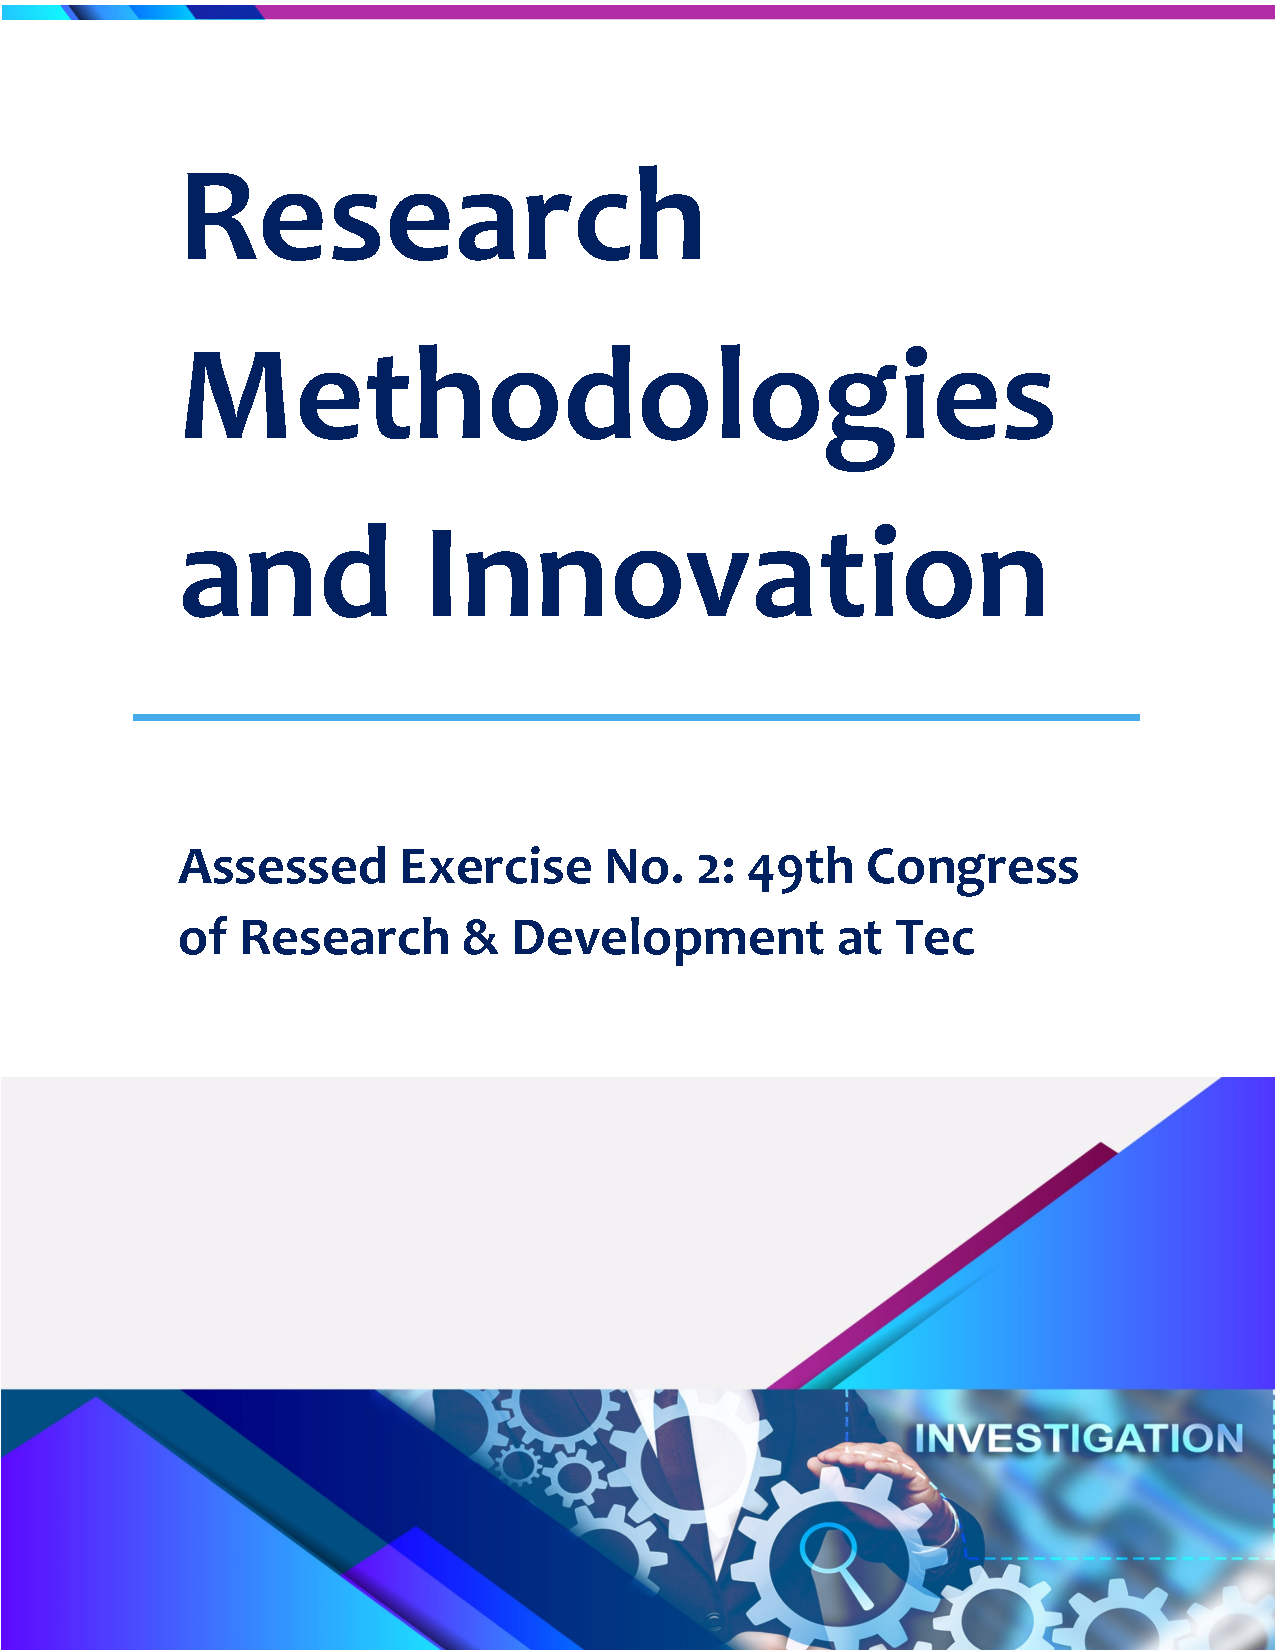
\includepdf[page=-]{pdf/MII-AssessedExercise02-201911}

%----------------------------------------------------------------------------------------%

\end{document}

%----------------------------------------------------------------------------------------%
